\chapter{Methodology}

\section{System Architecture}

Our image enhancement pipeline consists of four sequential stages: (1) image loading \& colour-space
preparation, (2) K-Means segmentation to produce per-region masks, (3) per-region
frequency-domain analysis using DFT and DCT, and (4) targeted filtering followed by
inverse transformation and channel blending. Figure~\ref{fig:pipeline} illustrates the
entire flow.


\begin{figure}
    \centering
    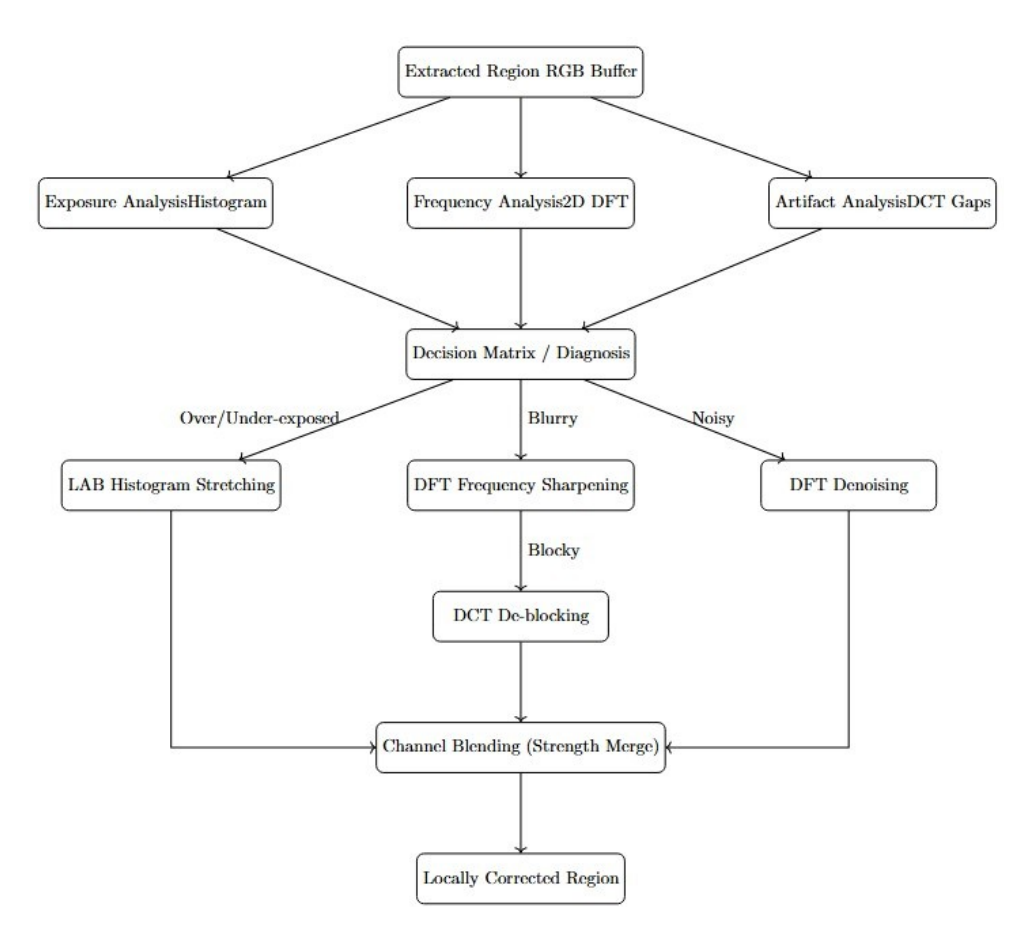
\includegraphics[width=1.0\linewidth]{images/flowchart.png}
    \label{fig:pipeline}
    \caption{Flow of our implementation}
    \label{fig:placeholder}
\end{figure}

\section{K-Means Segmentation}

K-Means is applied directly to the pixel colour vectors (R, G, B) of the input image. We begin the
algorithm by selecting $K$ random pixels as initial centroids. At each
iteration, every pixel is assigned to the cluster whose centroid is closest under the
Euclidean $L^2$ norm, and centroids are then recalculated as the arithmetic mean of all
assigned pixels. Iteration continues until the centroids do not change between next
steps (which means we've reached convergence).

\vspace{0.15in}
\noindent
The segmentation produces $K$ binary masks, one per cluster, which serve as region
selectors for all downstream processing. A configurable value of $K$ is exposed via
command-line argument, allowing the user to control segmentation granularity.


\begin{figure}[H]
    \centering
    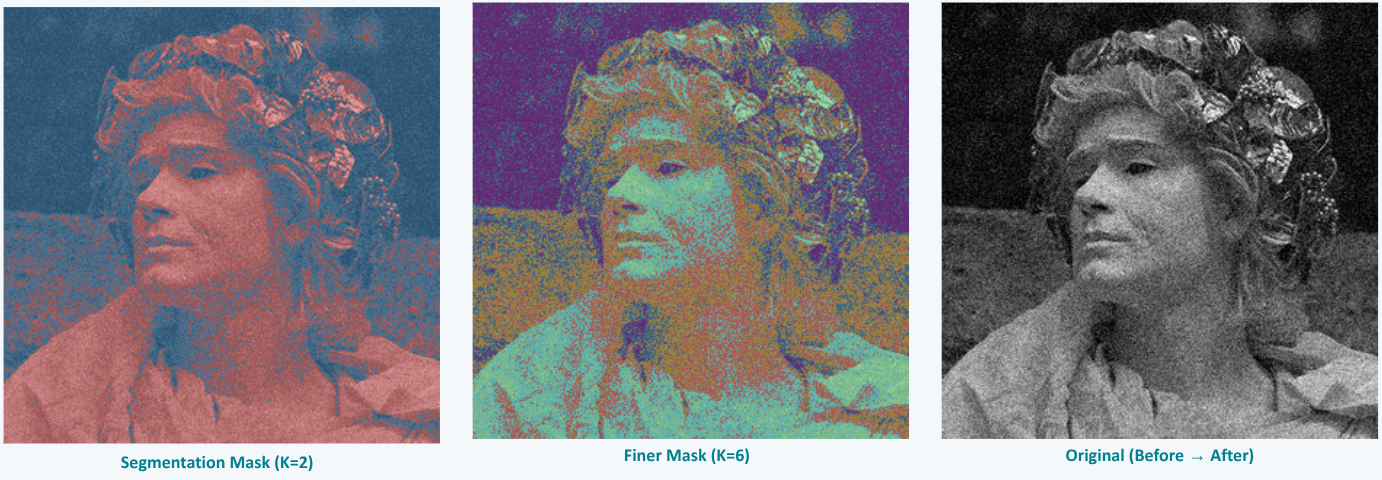
\includegraphics[width=\textwidth]{images/k-means.png}
    \caption{K-Means Segmentation}
    \label{fig:placeholder}
\end{figure}

\subsection{Removing JPEG artifacts with Inv. DCT}

When the DCT is applied to a segmented region, the
artificial boundaries producing high-energy responses in the frequency matrix
lights up the spectrum at positions corresponding to the boundary frequencies. so what we do is compare DCT spectra with \& without
segmentation-boundary smoothing, the system quantifies how much structural distortion
the K-Means step introduces.

\begin{figure}[H]
    \centering
    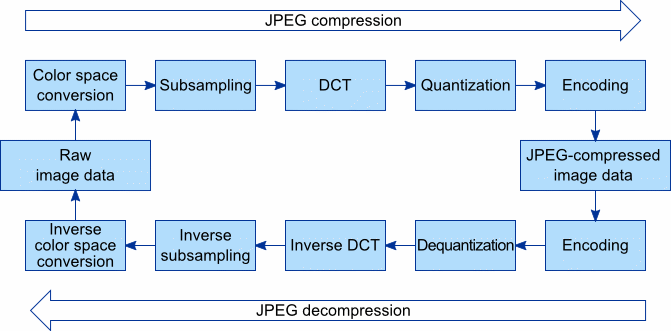
\includegraphics[width=0.75\linewidth]{images/idct.png}
    \label{fig:placeholder}
\end{figure}

\section{Frequency-Domain Filtering}

\subsection{Low-Pass Filtering}

Low-pass filters attenuate high-frequency components while preserving low-frequency
content, producing a smoothing effect. Applied to a K-Means cluster, a low-pass filter
suppresses intra-region noise but maintaining the cluster's overall shape and colour
distribution.


\subsection{High-Pass Filtering}

High-pass filters suppress low-frequency (smooth) content and retain high-frequency
(edge and detail) content. They have been used in our code to accentuate the boundaries between
K-Means clusters and to apply sharpening within a region.

\vspace{0.15in}
\noindent
Because high-pass and low-pass filters are complementary, the high-pass mask is derived
algebraically from the low-pass mask:

\begin{equation}
    H_{\text{HP}}(u,v) = 1 - H_{\text{LP}}(u,v)
\end{equation}


\begin{figure}[H]
    \centering
    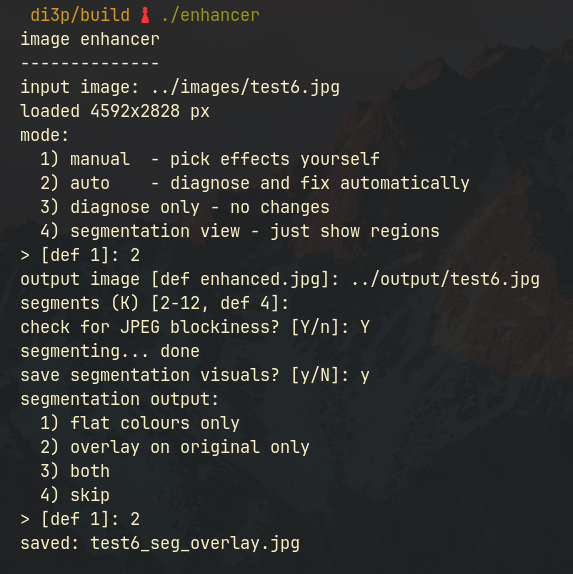
\includegraphics[width=0.75\linewidth]{images/dryrun.png}
    \caption{Sample Output of our workflow}
    \label{fig:placeholder}
\end{figure}
